% Created 2023-06-15 Thu 19:16
% Intended LaTeX compiler: pdflatex
\documentclass[9pt,twocolumn]{article}
\usepackage[utf8]{inputenc}
\usepackage[T1]{fontenc}
\usepackage{graphicx}
\usepackage{longtable}
\usepackage{wrapfig}
\usepackage{rotating}
\usepackage[normalem]{ulem}
\usepackage{amsmath}
\usepackage{amssymb}
\usepackage{capt-of}
\usepackage{hyperref}
\usepackage{algpseudocode}
\usepackage{algorithm}
\usepackage{cleveref}
\usepackage{amsthm}
\usepackage{pythonhighlight}
\usepackage{mdframed}
\BeforeBeginEnvironment{minted}{\begin{mdframed}}
\AfterEndEnvironment{minted}{\end{mdframed}}
\newtheorem{theorem}{Theorem}
\author{Barak-Nadav Diker}
\date{\today}
\title{Assignment 2}
\hypersetup{
 pdfauthor={Barak-Nadav Diker},
 pdftitle={Assignment 2},
 pdfkeywords={},
 pdfsubject={},
 pdfcreator={Emacs 28.2 (Org mode 9.6.1)}, 
 pdflang={English}}
\begin{document}

\maketitle


\section*{Question 1}
\label{sec:org027f6b0}

Given the following graph

\begin{center}
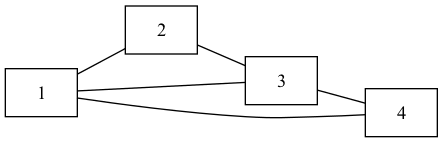
\includegraphics[width=.9\linewidth]{Question1_graph.png}
\end{center}

Calculate all walks of size 6 in the given graph


\subsection*{Answer}
\label{sec:orgb52fa78}
In order to do so we'll use the following theorem

\begin{theorem} [ Walks Theorem ]
If A is the adjacency matrix of a graph or digraph G with vertices \( \{v1, . . . vn\} \), then the i, j entry
of \(A^k\) is the number of walks of length k from \(v_i\) to \(v_j\)
\label{theorem:walk}
\end{theorem}

By \ref{theorem:walk} we can just multiple the adjacency matrix by itself 6 times
and we'll get all the walks available from node i into node j

Since the problem specify undirected graph we'll have to sum all elements of the matrix and divide it by 2

\newpage
\begin{algorithm}
\caption{All walks of length 6 }
\begin{algorithmic}
\State \(n \gets 6 \) \Comment{6 => length of walk}
\State \( Adj  \) \Comment{adjacency matrix}
\State \( M \gets I \)
\While{ \(n \neq 0 \) }
\State \( M \gets M \times Adj \) \Comment{Matrix Multiples}
\EndWhile
\State \( sum \gets 0 \)
\While{ $a \in M $}
\State \( sum \gets sum + a \)
\EndWhile
\end{algorithmic}
\label{algo:walk}
\end{algorithm}

We will apply \textbf{algorithm} \ref{algo:walk}  for getting the number of walk of length 6

\phantomsection
\label{calculate:walks}
\begin{python}
import numpy
from numpy.linalg import matrix_power
input_array = numpy.array([[0,1,1,1],
                           [1,0,1,0],
                           [1,1,0,1],
                           [1,0,1,0]])
A_to_power6 = matrix_power(input_array, 6)
sum_var = 0
for row in A_to_power6:
    for elem in row:
        sum_var += elem
int(sum_var/2)
# output is 557
\end{python}



\section*{Question 2}
\label{sec:org1d26e99}
Consider the following quote
\begin{quote}
``Undirected Graph can be considered as directed graph''
\end{quote}
Prove it

Formally , Given an Undirected graph find a directed graph such that \(A_G = A_{G'}\)


\subsection*{Answer}
\label{sec:org86b991f}
Given An undirected graph mark it \(G=(V,E)\) and the adjacency matrix of his as \(A_G\)

Define the directed graph \(G'=(V',E')\) where \(V'=V\) and

\[ \forall e=(v_1,v_2)\in E : e_1=(v_1,v_2) , e_2=(v_2,v_1)\in E'  \]

The adjancey matrix of the directed graph is equal to the adjancey matrix of the undirected graph

\[ A_G=A_{G'} \]



\section*{Question 3}
\label{sec:orgc997ab0}
Prove that given a directed graph \(G=(V,E)\) where \(V=(1,2,..,n)\) , let A be the adjacency matrix
\[ l \in \mathbb{N}\cap{\{0\}}: \forall i,j\in V : F(j,i ,l)=(A^l)_{i,j} \]
where \(F:V \times V \times \mathbb{N}\cap{\{0\}} \rightarrow \mathbb{N}\cap{\{0\}}\)
are all the walks from node j to i of length l

\subsection*{Answer}
\label{sec:org25e04e8}
We'll prove the theorem by induction
\begin{proof}
By induction

\underline{\textbf{Base Case:}}
For k = 1, \( A^k = A \), and there is a walk of length 1 between i and j
if and only if \(a_{ij} = 1\), thus the result holds.


\underline{\textbf{Step Case:}}
Assume the proposition holds for
\( k = n \) and consider the matrix \( A_{n+l} = A_nA \), By the inductive hypothesis, the
\( (i,j)^{th} \) entry of \( A_n \) counts the number of walks of length n between vertices i
and j. Now, the number of walks of length n + 1 between i and j equals the
number of walks of length n from vertex i to each vertex v that is adjacent to j.
But this is the \( (i,j)^{th} \) entry of \( A^nA = A^{n+1} \) the non-zero entries of the column
of A corresponding to v are precisely the first neighbours of v. Thus the result
follows by induction on n
\end{proof}

\section*{Question 4}
\label{sec:orgf491d3e}
Find the number of possible walks of length 8 from 1 to 4 by the following undirected graph

\begin{center}
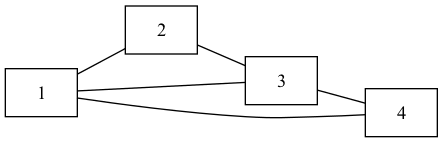
\includegraphics[width=.9\linewidth]{Question1_graph.png}
\end{center}
\subsection*{Answer}
\label{sec:org9fc08d1}
We'll Write the adjancey matrix and calculate the \(A^8\)

To do so we'll use the same code

\phantomsection
\label{calculate:question4:walks}
\begin{python}
import numpy
from numpy.linalg import matrix_power
input_array = numpy.array([[0,1,1,0],
                           [0,0,0,1],
                           [1,1,0,0],
                           [1,0,1,0]])
A_to_power6 = matrix_power(input_array, 8)
A_to_power6[3][0]
# output is 23
\end{python}

\section*{Introduction}
\label{sec:orgf6d9620}
Kruskal's algorithm[1] finds a minimum spanning forest of an undirected edge-weighted graph. If the graph is connected, it finds a minimum spanning tree. (A minimum spanning tree of a connected graph is a subset of the edges that forms a tree that includes every vertex, where the sum of the weights of all the edges in the tree is minimized. For a disconnected graph, a minimum spanning forest is composed of a minimum spanning tree for each connected component.) It is a greedy algorithm in graph theory as in each step it adds the next lowest-weight edge that will not form a cycle to the minimum spanning forest.[2]



This algorithm first appeared in Proceedings of the American Mathematical Society, pp. 48–50 in 1956, and was written by Joseph Kruskal.[3] It was rediscovered by Loberman \& Weinberger (1957).[4]

Other algorithms for this problem include Prim's algorithm, the reverse-delete algorithm, and Borůvka's algorithm.


\section*{Simple pseudo code}
\label{sec:org5c3a5bb}
Here is some code

This is some random text



\begin{mdframed}
\begin{algorithmic}
\State $i \gets 10$
\If{$i\geq 5$}
    \State $i \gets i-1$
\Else
    \If{$i\leq 3$}
        \State $i \gets i+2$
    \EndIf
\EndIf
\end{algorithmic}
\end{mdframed}

bla bla bla


Another Example , please note the following


\begin{algorithm}
\caption{An algorithm with caption}\label{alg:cap}
\begin{algorithmic}
\Require $n \geq 0$
\Ensure $y = x^n$
\State $y \gets 1$
\State $X \gets x$
\State $N \gets n$
\While{$N \neq 0$}
\If{$N$ is even}
    \State $X \gets X \times X$
    \State $N \gets \frac{N}{2}$  \Comment{This is a comment}
\ElsIf{$N$ is odd}
    \State $y \gets y \times X$
    \State $N \gets N - 1$
\EndIf
\EndWhile
\end{algorithmic}
\end{algorithm}
\end{document}